%%%%%%%%%%%%%%%%%%%%%%%%%%%%%%%%%%%%%%%%%%%%%%%%%%%%%%%%%%%%%%%%%%%%%%
%%%%%%%%%  TEMPLATE IEEE PARA ENTREGA DEL ARTÍCULO FINAL DE  %%%%%%%%% 
%%%% PRÁCTICA DE INGENIERÍA ELECTRÓNICA DE LA UNIVERSIDAD CENTRAL %%%%
%%%%%%%%%%%%%%%%%%%%%%%%    BOGOTÁ, COLOMBIA    %%%%%%%%%%%%%%%%%%%%%%
%%%%%%%%%%%%%%%%%%%%%%%%%%%%%%%%%%%%%%%%%%%%%%%%%%
%%%%   AUTOR: SERGIO ANDRÉS CHAPARRO MORENO   %%%%
%%%%%%%%%%%%%%%%%%%%%%%%%%%%%%%%%%%%%%%%%%%%%%%%%%
%%%%%%%%%%%%%  VERSIÓN 1.0-ENE 2017  %%%%%%%%%%%%%
%%%%%%%%%%%%%%%%%%%%%%%%%%%%%%%%%%%%%%%%%%%%%%%%%%
\documentclass[journal]{IEEEtran}
\IEEEoverridecommandlockouts
%%%%%%%%%%%%%%%%%%%%%%%%%%%%%%%%%%%%%%
%%%%%%%% PRINCIPALES PAQUETES %%%%%%%%
%%%%%%%%%%%%%%%%%%%%%%%%%%%%%%%%%%%%%%
\usepackage{float}
\restylefloat{table}
\usepackage[table]{xcolor}% http://ctan.org/pkg/xcolor
\usepackage{fancyhdr}
\usepackage{graphicx}
\usepackage[spanish, es-tabla]{babel}
\usepackage[utf8]{inputenc}
\usepackage{color}
\usepackage{hyperref}
\usepackage{wrapfig}
\usepackage{array}
\usepackage{multirow}
\usepackage{adjustbox}
\usepackage{nccmath}
%\usepackage{anysize}
\usepackage{subfigure}
\usepackage{amsfonts,latexsym} % para tener disponibilidad de diversos simbolos
\usepackage{enumerate}
\usepackage{booktabs}
\usepackage{float}
\usepackage{threeparttable}
\usepackage{array,colortbl}
\usepackage{ifpdf}
\usepackage{rotating}
\usepackage{cite}
\usepackage{stfloats}
\usepackage{url}
\usepackage{listings}
%%%%%%%%%%%%%%%%%%%%%%%%%%%%%%%%%%%%%%%%%%%
%%% CREAR Y REESCRIBIR ALGUNOS COMANDOS %%%
%%%%%%%%%%%%%%%%%%%%%%%%%%%%%%%%%%%%%%%%%%%
\newcolumntype{P}[1]{>{\centering\arraybackslash}p{#1}}  %% Se crea un nuevo tipo de columna llamada P.
\newcommand{\tabitem}{~~\llap{\textbullet}~~}
\newcommand{\ctt}{\centering\scriptsize\textbf} %%\ctt abrevia el comando \centering\scriptsize\textbf
\newcommand{\dtt}{\scriptsize\textbf} %%\dtt abrevia el comando \scriptsize\textbf
\renewcommand\IEEEkeywordsname{Palabras clave}
%%%%%%%%%%%%%%%%%%%%%%%%%%%%%%%%%%%%%%%%%%%


% correct bad hyphenation here
\hyphenation{op-tical net-works semi-conduc-tor} %% Con este comando se especifican como pueden seprarse las sílabas adecuadamente en caso una palabra quede en dos lineas diferentes de texto

\graphicspath{ {Figs/} }  %%Ruta donde se encuentran las imágenes, que esté vacio indica que las imagenes están dentro de la misma carpeta que contiene el archivo .tex


%%%%%%%%%%%%%%%%%%%%%%%%%%%%%%%%%%%%%%%%%%%%%%%%%%%%%%%%%%
%%% ENCABEZADO DE LAS PÁGINAS TIPO UNIVERSIDAD CENTRAL %%%
%%%%%%%%%%%%%%%%%%%%%%%%%%%%%%%%%%%%%%%%%%%%%%%%%%%%%%%%%%
\newcommand{\MYhead}{\smash{\scriptsize
\hfil\parbox[t][\height][t]{\textwidth}{\centering
\begin{picture}(0,0) \put(-0,-15){
\includegraphics[width=50mm]{Imagenes/dfi.pdf}} \end{picture} \hspace{6.4cm}
UNIVERSIDAD DE CHILE
\hspace{5.15cm} Versión 1.0\\
\hspace{6.4cm} DEPARTAMENTO DE FÍSICA 
\hspace{5cm} Otoño 2021\\
\underline{\hspace{ \textwidth}}}\hfil\hbox{}}}
\makeatletter
% normal pages
\def\ps@headings{%
\def\@oddhead{\MYhead}%
\def\@evenhead{\MYhead}}%
% title page
\def\ps@IEEEtitlepagestyle{%
\def\@oddhead{\MYhead}%
\def\@evenhead{\MYhead}}%
\makeatother
% make changes take effect
\pagestyle{headings}
% adjust as needed
\addtolength{\footskip}{0\baselineskip}
\addtolength{\textheight}{-1\baselineskip}
%%%%%%%%%%%%%%%%%%%%%%%%%%%%%%%%%%%%%%%%%%%%%%%%%%%%%%%%%%
%%%%%%%%%%%%%%%%%%%%%%%%%%%%%%%%
%%%%% INICIO DEL DOCUMENTO %%%%%
%%%%%%%%%%%%%%%%%%%%%%%%%%%%%%%%
\begin{document}
%%%%%%%%%%%%%%%%%%%%%%%%%%%%
%%% TÍTULO DEL DOCUMENTO %%%
%%%%%%%%%%%%%%%%%%%%%%%%%%%%
\title{Formación de una película de aluminio conductora}
%%%%%%%%%%%%%%%%%%%%%%%%%%%%
%%%%%%%%% AUTORES %%%%%%%%%
%%%%%%%%%%%%%%%%%%%%%%%%%%%
\author{Méndez~Matías~y~
        Villar~Gustavo~\\
				\textit{\{matías.mendez~y~gustavo.villar\}@ug.uchile.cl}\\
				Profesores:~Falcón~Claudio~y~Fuenzalida~Víctor\\
				Profesores Auxiliares:~Contreras~Consuelo~y~González~Gregorio}
% \thanks{El presente documento corresponde al informe de la unidad 2 de Física Experimental I, cual fue hecho gracias a la gratuidad, sin ella probablemente ni siquiera estaría estudiando. Gracias también a la primera línea, porque lo entendieron todo.}} %\thanks anexa una nota a pie de página donde se puede colocar alguna información sobre la naturaleza del documento.
% %%%%%%%%%%%%%%%%%%%%%%%%%%%

% Comando que indica la generación del título
\maketitle

%%%%%%%%%%%%%%%%%%%%%
%%%%%% RESUMEN %%%%%%
%%%%%%%%%%%%%%%%%%%%%
\begin{abstract}
% En este documento se presenta una plantilla elaborada en \LaTeX para la presentación del documento final, como producto del desarrollo de la asignatura práctica de ingeniería electrónica. En esta sección se espera el resumen del problema, la solución propuesta y los principales resultados alcanzados.
En este documento se presenta el informe sobre la evaporación de aluminio, correspondiente a la unidad 2 sobre vacío del curso de Física Experimental I. Se presenta el montaje del experimento realizado a partir de un sistema de vacío, para llegar a evaporar una película de aluminio y lograr que conduzca electricidad.
\end{abstract}
% En el resumen no se recomienda colocar citaciones bibliográficas.
%%%%%%%%%%%%%%%%%%%%%%
%%% PALABRAS CLAVE %%%
%%%%%%%%%%%%%%%%%%%%%
\begin{IEEEkeywords}
vacío, aluminio, bomba difusora, bomba rotatoria, termocupla, válvula, cámara, temperatura, presión, electricidad, vidrio. 
\end{IEEEkeywords}
%%%%%%%%%%%%%%%%%%%%%
%\IEEEpeerreviewmaketitle
%%%%%%%%%%%%%%%%%%%%%%%%%%%%%%%%%%%%%
%%% PRIMERA SECCIÓN DEL DOCUMENTO %%%
%%%%%%%%%%%%%%%%%%%%%%%%%%%%%%%%%%%%%
\section{Introducción}

Las láminas delgadas son capas de material depositadas sobre un sustrato, estas pueden variar desde nanómetros hasta varios micrómetros de espesor. Las láminas delgadas permiten mejorar las propiedades superficiales del sustrato u otorgarlas en caso que no las posea. Algunas de estas propiedades pueden ser transmisión, reflexión, absorción, dureza, resistencia a la abrasión, corrosión, permeación y comportamiento eléctrico. 

Las propiedades que pueden otorgar tienen una amplia gama de aplicaciones principalmente en la industria óptica y electrónica. Algunos ejemplos de aplicaciones son, regulación de adhesión celular a superficies; fabricación de maquinas y herramientas de corte; componentes ópticos; dispositivos electrónicos; superficies bidimensionales (almacenamiento magnético de datos); monitores; sensores; generación de energía (celdas fotovoltaicas). 

Por sus aplicaciones, existe un gran interés en la industria por encontrar métodos alternativos que puedan ser menos costosos, más confiables o capaces de producir películas con propiedades nuevas o mejoradas.

%%%%%%%%%%%%%%%%%%%%%%%%%%%%%%%%%%%%%
%%%%% SECCIONES DE MARCO TEÓRICO %%%%
%%%%%%%%%%%%%%%%%%%%%%%%%%%%%%%%%%%%%
\section{Metodología}	

Con el objetivo de conseguir un alto vacío, se monta un sistema de vacío. 
Este montaje consiste en una cámara de vacío, una bomba rotatoria, una bomba difusora y medidores de presión.  Como se puede ver en la figura \ref{figura montaje}.  \\

En la cámara de vacío hay un circuito abierto y un soporte para sujetar un portaobjetos. Este circuito esta alimentado por un transformador y se puede regular la corriente que lo circula a través de una manilla, esta corriente es medida con un amperímetro. \\ 

En el experimento se utiliza un alambre de tungsteno de 0.5 mm de diámetro, un portaobjetos de vidrio, una máscara de molibdeno y trozos de aluminio.\\

Se comienza limpiando la lámina de vidrio y la máscara. Primero con acetona y luego con etanol para quitar la acetona. Esto se hace para quitar impurezas que contaminen la cámara. Luego se deja secar en papel sin pelusa. Después se abre la válvula 5 para evacuar la cámara, y abrirla. \\ 

Se enrolla el alambre de tungsteno en forma de hélice. Se cierra el circuito con el alambre y se colocan tres pedazos de aluminio doblados de forma que queden sujetos al alambre.
Se ubica la máscara en la lámina de vidrio y ambas se colocan en el soporte de forma que la normal a su cara frontal apunte hacia el alambre con el aluminio. 
Se coloca la cámara y la malla de seguridad. Y se procede a cerrar todas las válvulas.\\

Luego se energiza el sistema y se enciende la bomba rotatoria. 

Se abre la válvula 3 para hacer un prevacío en la cámara.
Cuando en la cámara se alcanza una presión de 1 Pa medido en el convectrón se cierra la válvula 3, y se abre la válvula 1 para hacer un prevacío en la bomba difusora.
Cuando el medidor termopar mide 20 Pa, se comienza a calentar el aceite de la bomba difusora. Se vuelve a hacer un prevacío en la cámara cerrando la válvula 1 y abriendo la válvula 3.
Se activa la trampa fría. 
\begin{figure}[H]
    \centering
    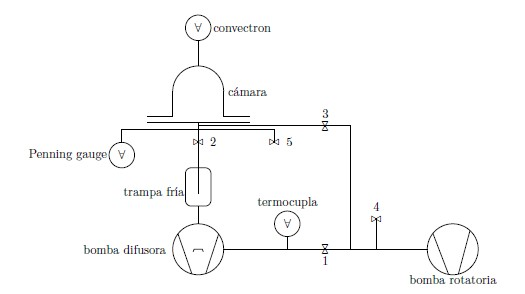
\includegraphics[width=0.5\textwidth]{Imagenes/p40.jpg}
    \caption{Esquema del montaje a utilizar. En las lineas que conectan los elementos del sistema se pueden apreciar las válvulas, enumeradas del 1 al 5.}
    \label{figura montaje}
\end{figure}

Después con un termopar se mide la temperatura de la bomba difusora, al alcanzar 138 °C se espera 20 minutos para que la presión bajo la válvula 2 sea menor que la presión en la cámara.
Cuando la temperatura llega a 142 °C se abre la válvula 2 y se vacía la cámara. \\

Al alcanzar una presión de $10^{-2}$ Pa en el medidor Penning, se baja la manilla al mínimo nivel y se enciende el transformador.
Se aumenta la corriente de forma gradual a una tasa de 1 A por minuto. Se alcanza una corriente de 20 A de forma que el aluminio se evapore. Se apaga el transformador. \\

Se cierra la válvula 2 y se apaga la bomba difusora. La trampa fría se apaga cuando el aceite llegue a 40 °C. 
Luego se cierra la válvula 4 y se apaga la bomba rotatoria. Se corta la corriente del sistema.
Se evacua la cámara abriendo la válvula 5 y se abre. Con un multímetro se prueba si la placa conduce.


\section{Resultados}
\begin{table}[H]
\centering
\begin{tabular}{|c|c|}
\hline
\textbf{Tiempo (min)} & \textbf{Presión  (Pa)} \\ \hline
0 & \cellcolor[HTML]{38FFF8}$8.1\cdot 10^{4}$ \\ \hline
2 & \cellcolor[HTML]{38FFF8}$1.6\cdot 10^3$ \\ \hline
4 & \cellcolor[HTML]{38FFF8}$74$ \\ \hline
7 & \cellcolor[HTML]{38FFF8}$26$ \\ \hline
9 & \cellcolor[HTML]{38FFF8}$23$ \\ \hline
12 & \cellcolor[HTML]{38FFF8}$21$ \\ \hline
17 & \cellcolor[HTML]{38FFF8}$20$ \\ \hline
22 & \cellcolor[HTML]{38FFF8}$20$  \\ \hline
27 & \cellcolor[HTML]{38FFF8}$19$ \\ \hline
32 & \cellcolor[HTML]{38FFF8}$19 $ \\ \hline
38 & \cellcolor[HTML]{38FFF8}$18 $ \\ \hline
43 & \cellcolor[HTML]{38FFF8}{\color[HTML]{000000} $18$} \\ \hline
47 & \cellcolor[HTML]{38FFF8}{\color[HTML]{000000} $18 $} \\ \hline
54 & \cellcolor[HTML]{38FFF8}{\color[HTML]{000000} $17 $} \\ \hline
72 & \cellcolor[HTML]{CD84B0}{\color[HTML]{000000} $36$} \\ \hline
77 & \cellcolor[HTML]{38FFF8}{\color[HTML]{000000} $18$} \\ \hline
207 & \cellcolor[HTML]{38FFF8}{\color[HTML]{000000} $27 $} \\ \hline
212 & \cellcolor[HTML]{F8A102}{\color[HTML]{000000} $2.30 \cdot 10^{-1}$} \\ \hline
249 & \cellcolor[HTML]{F8A102}{\color[HTML]{000000} $2.1 \cdot 10^{-2}$} \\ \hline
262 & \cellcolor[HTML]{F8A102}{\color[HTML]{000000} $2.0 \cdot 10^{-2}$} \\ \hline
\end{tabular}
\caption{Medición de la presión de la cámara a través del tiempo. El color celeste muestra las mediciones hechas por el termopar, en morado se tiene la cámara aislada y en naranjo las mediciones del medidor Penning.}
\label{tabla con colores}
\end{table}
 
 
 \begin{figure}[H]
    \centering
    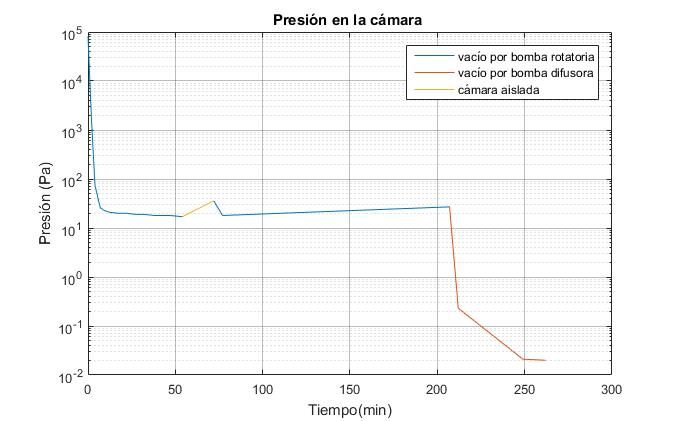
\includegraphics[width=0.5\textwidth]{Imagenes/graf1.jpg} 
    \caption{Gráfico de la presión medida en la cámara versus tiempo. }
    \label{grafico presion en la camara }
\end{figure}


\begin{table}[H]
\centering
\resizebox{0.3\textwidth}{!}{%
\begin{tabular}{|c|c|c|}
\hline
\textbf{Tiempo (min)} & \textbf{Temperatura (C)} & \textbf{Presión (Pa)} \\ \hline
0 & * & $27$  \\ \hline
3 & * & $22 $ \\ \hline
6 & * & $21$ \\ \hline
10 & * & $20 $ \\ \hline
18 & 31 & $35 $ \\ \hline
20 & 43 & $32 $ \\ \hline
25 & 76 & $29 $ \\ \hline
30 & 108 & $35 $ \\ \hline
35 & 127 & $29 $ \\ \hline
40 & 134 & $23 $ \\ \hline
45 & 140 & $21$ \\ \hline
50 & 142 & $20 $ \\ \hline
55 & 142 & $19 $ \\ \hline
60 & 142 & $19 $ \\ \hline
65 & 143 & $19 $ \\ \hline
70 & 140 & $17 $ \\ \hline
80 & 141 & $17 $ \\ \hline
95 & 140 & $16 $ \\ \hline
113 & 143 & $16 $ \\ \hline
\end{tabular}}
\caption{Medición de la presión y temperatura del aceite en la bomba difusora.}
\label{tabla temperatura y presion}
\end{table}
 
\begin{figure}[H]
    \centering
    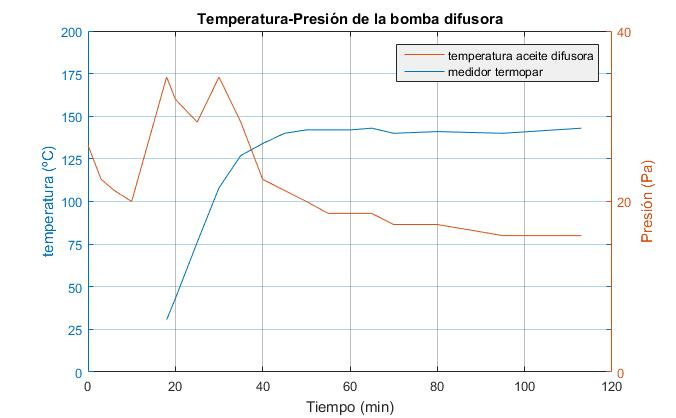
\includegraphics[width=0.5\textwidth]{Imagenes/graf2.jpg}
    \caption{Gráfico de la presión y temperatura medida del aceite en la bomba difusora.}
    \label{grafico presion temperatura}
\end{figure}
 
 
 
 \begin{table}[H]
\centering
\resizebox{0.2\textwidth}{!}{%
\begin{tabular}{|c|c|}
\hline
\textbf{Tiempo  (min)} & \textbf{Corriente (A)} \\ \hline
0                      & 1.8                    \\ \hline
2                      & 2.4                    \\ \hline
3                      & 3.3                    \\ \hline
5                      & 3.5                    \\ \hline
6                      & 4.1                    \\ \hline
7                      & 4.6                    \\ \hline
8                      & 5.1                    \\ \hline
10                     & 5.7                    \\ \hline
12                     & 6.5                    \\ \hline
13                     & 7.2                    \\ \hline
14                     & 7.8                    \\ \hline
15                     & 8.5                    \\ \hline
17                     & 9.0                     \\ \hline
18                     & 9.9                    \\ \hline
20                     & 10.8                   \\ \hline
21                     & 10.5                   \\ \hline
23                     & 11.7                   \\ \hline
24                     & 12.0                    \\ \hline
24                     & 12.5                   \\ \hline
26                     & 12.5                   \\ \hline
27                     & 13.1                   \\ \hline
28                     & 13.7                   \\ \hline
29                     & 14.7                   \\ \hline
30                     & 15.2                   \\ \hline
31                     & 15.9                   \\ \hline
32                     & 16.4                   \\ \hline
33                     & 17.5                   \\ \hline
34                     & 18.4                   \\ \hline
36                     & 20.1                   \\ \hline
\end{tabular}}
\caption{Medición de la corriente en el circuito.}
\label{tabla amperes}
\end{table}
 
 
 Haciendo uso de un multímetro se detecta conducción eléctrica en la película de aluminio.

\section{Análisis}
En la tabla \ref{tabla con colores} se aprecia la presión de la cámara representada en la figura \ref{grafico presion en la camara }, en esta se puede observar que cuando la cámara se aísla la presión dentro de esta aumenta. Además la presión alcanzada por la bomba rotatoria converge con el tiempo.

En la tabla \ref{grafico presion temperatura} se aprecia la presión y temperatura de la bomba difusora representadas en el gráfico \ref{grafico presion temperatura}, en el cual se observa que en el momento que se enciende la bomba difusora se detecta un aumento en la presión medida por el termopar.

En el experimento, como se observa en la tabla \ref{tabla amperes}, ocurrió un aumento espontáneo de la corriente en el circuito entre los 8 A y 10 A.

\section{Discusión }
El aumento de la presión en la cámara aislada se debe a flujos de fuga presentados por problemas en los equipos, es probable que hayan fugas en el sistema.

El aumento de la presión medida por el termopar es resultado del bombeo de partículas de la cámara por la bomba difusora. Se produce un aumento en el número de partículas circulando por la conexión entre la bomba difusora y la rotatoria, esto explica el aumento de presión detectado.

La corriente aumenta espontáneamente debido a que la tensión superficial del aluminio permite que este se extienda por todo el alambre modificando la resistencia del circuito. \\

Si bajo la válvula 2 se mantiene una presión similar que en la cámara antes de abrir la válvula, el vacío de la cámara toma más tiempo. Mas aún, si es mayor a la presión en la cámara se puede producir una corriente de retorno que contamine la cámara. De esta manera si la presión bajo la válvula 2 es menor que en la cámara, esta última se vaciará más rápido.

La película resultante logra conducir la electricidad porque el vacío permite que llegue la cantidad suficiente de aluminio al sustrato, además de conseguir una superficie limpia de impurezas.

\section{Conclusiones}
Se consigue formar una película delgada de aluminio que conduce la electricidad.

El sistema de vacío compuesto por una bomba rotatoria y una bomba difusora permite generar un alto vacío.

El alto vacío permite generar superficies limpias y construir películas delgadas de material.\\

El hecho que los equipos no estén en óptimo estado dificulta la obtención de vacío y además impide recuperar los elementos de la cámara manteniendo el vacío en la bomba difusora. Por lo que el vacío se puede generar de forma mas rápida y eficiente con un equipo en óptimas condiciones.

La manilla que permite el paso de la corriente es muy sensible lo que puede provocar un aumento excesivo en la corriente y cortar el alambre. Por lo que utilizar un regulador menos sensible puede evitar este problema.



%%%%%%%%%%%%%%%%%%%%%%%%%%%%%%
%%%%% CITAR BIBLIOGRAFIA %%%%%
%%%%%%%%%%%%%%%%%%%%%%%%%%%%%%
% \subsection{Citar en formato IEEE}
% Para citar referencias bibliográficas se usa el comando cite. En \cite{nombre_para_citar} se muestran los campos que deben llenarse en una referencia, en \cite{kopka} se muestra un ejemplo, y en \cite{link} se muestra como citar un enlace. Preferiblemente citar libros y artículos.
%%%%%%%%%%%%%%%%%%%%%%%%%%%%%%
%%%%%%%%%%%%%%%%%%%%%%%%%%%%%%%%%%%%%%%%%%%%%%
%%%%%% SECCIONES DE DISEÑO Y DESARROLLO %%%%%%
%%%%%%%%%%%%%%%%%%%%%%%%%%%%%%%%%%%%%%%%%%%%%%


%%%%%%%%%%%%%%%%%%%%%%%%%%%%%%%%%%%%%

\ifCLASSOPTIONcaptionsoff
  \newpage
\fi

%%%%%%%%%%%%%%%%%%%%%%%%%%
%%%%%% BIBLIOGRAFIA %%%%%%
%%%%%%%%%%%%%%%%%%%%%%%%%%
\begin{thebibliography}{1}

% \bibitem{nombre_para_citar}
% Inicial1.~Apellido1 and Inicial2.~Apellido2, \emph{Nombre de libro}, \#edición~ed.\hskip 1em plus
%   0.5em minus 0.4em\relax Ciudad, País: Editorial, año.

\bibitem{nombre_para_citar}
J. F.~ O´Hanlon, \emph{A User's Guide to Vacuum Technology}, 3rd ed.\hskip 1em plus
0.5em minus 0.4em\relax New Jersey, United States of America: Jhon Wiley & Sons, 2003.
\\	
\bibitem{nombre_para_citar}
H.~Frey and H.R.~Khan, \emph{Handbook of Thin-Film Technology}, \hskip 1em plus 
0.5em minus 0.4em\relax Springer, 2015.
\url{https://doi.org/gjxv}
\\
\bibitem{nombre_para_citar}
J.I.~Brauman and P.~Szuromi, Thin films, \emph{Science, 273}(5277), 855.\hskip 1em plus
0.5em minus 0.4em\relax 1996.
\url{https://doi.org/fdkhnh}

\end{thebibliography}
%%%%%%%%%%%%%%%%%%%%%%%%%%

\end{document}
%%%%%%%%%%%%%%%%%%%%%%%%%%%%%%%%
%%%%%% FIN DEL DOCUMENTO %%%%%%%
%%%%%%%%%%%%%%%%%%%%%%%%%%%%%%%%




